\documentclass[border={1cm 0.5cm 1cm -1.25cm}]{standalone}  %E,S,W,N

\usepackage{amssymb}
\usepackage{amsmath}
\usepackage{tikz}

%“The coincidence effect,” from Taylor, Rupert. (1970). Noise. New York: Penguin, fig. 41

%Note: this takes a long time to compile, because of all of the random dots
%increasing the density would make it look nicer, but who's got that kind of time?

\begin{document}
	
	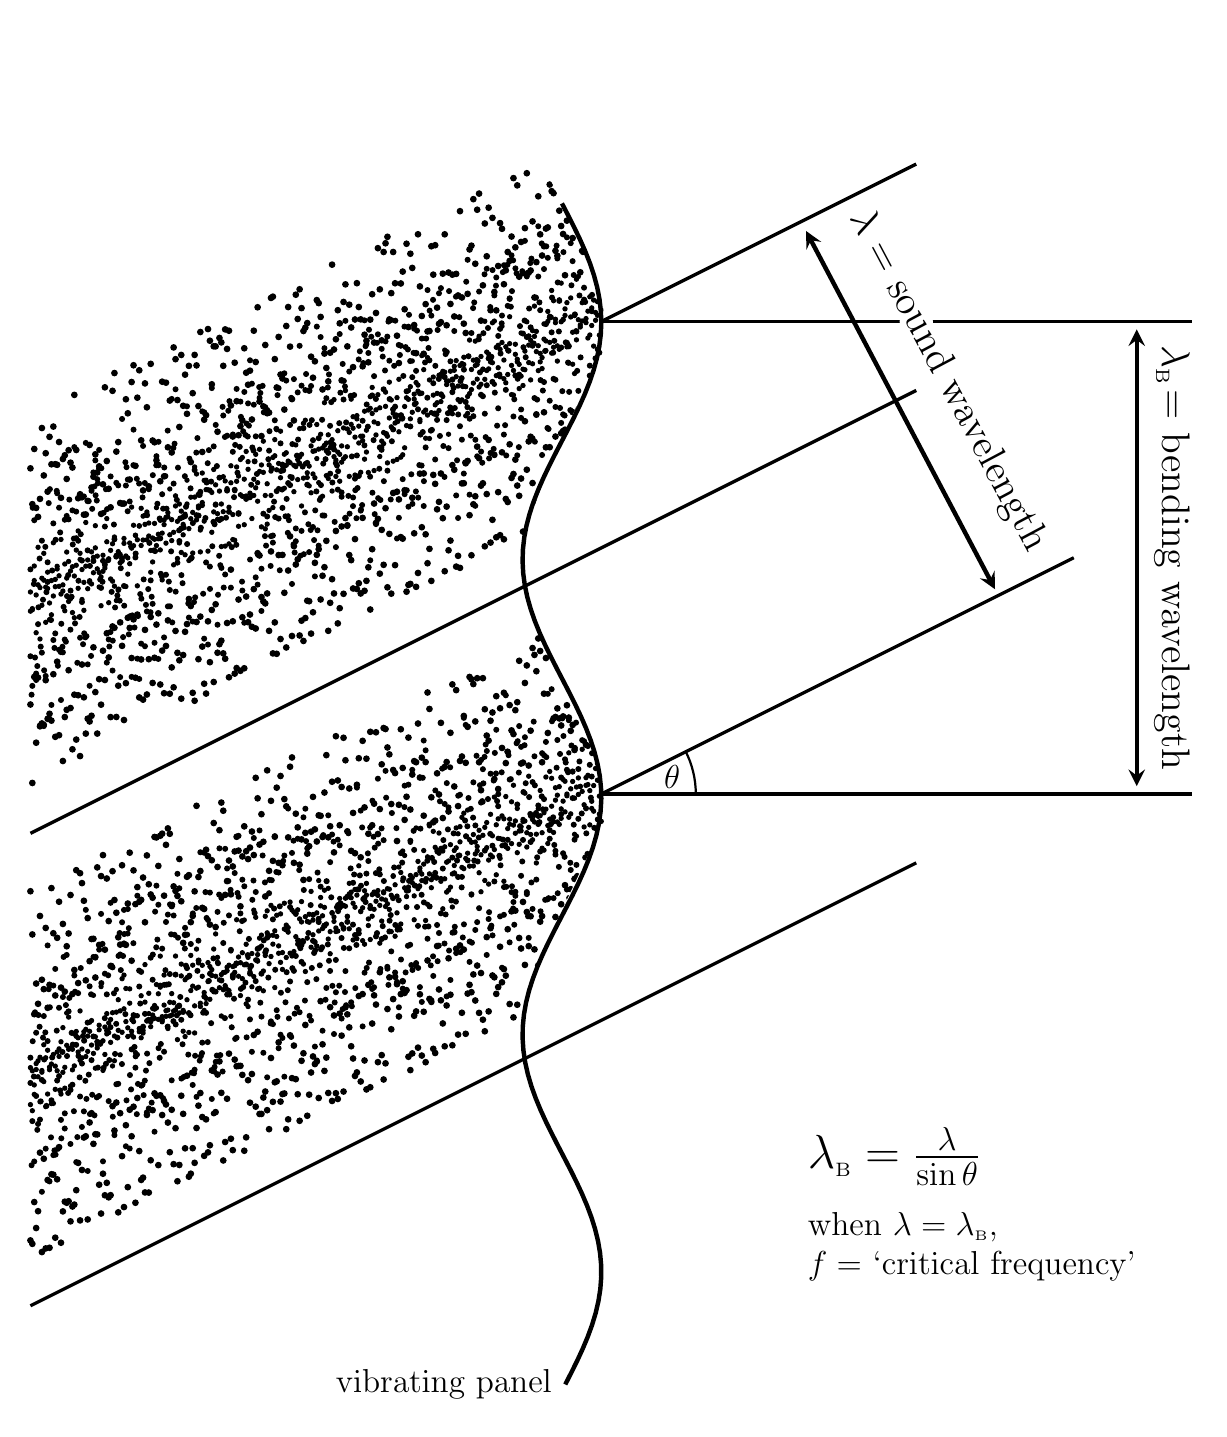
\begin{tikzpicture}
	%RANDOM DOTS (total: 2800)
	%based on https://tex.stackexchange.com/questions/145969
	\draw[domain=-7.25:0,only marks,mark=*,samples=300,mark size=1] plot (\x,{0.5*6+0.5*9.125+0.5*\x + 0.5*rand*-1.75});	%large dots, upper band
	\draw[domain=-7.25:0,only marks,mark=*,samples=300,mark size=1] plot (\x,{0.5*6+0.5*3+0.5*\x+0.5*rand*-1.5});	%large dots, lower band
%%	\draw[domain=-7.25:0,only marks,mark=*,samples=300,mark size=1] plot (\x,{0.5*3.125+0.5*9.125+0.5*\x + 0.5*rand*-4.5});	%large dots
	\draw[domain=-7.25:0,only marks,mark=*,samples=300,mark size=0.875] plot (\x,{0.5*3.125+0.5*9.125+0.5*\x + 0.5*rand*-3.5});	%big dots
	\draw[domain=-7.25:0,only marks,mark=*,samples=500,mark size=0.875] plot (\x,{0.5*3.125+0.5*9.125+0.5*\x + 0.5*rand*-2.5});	%medum dots
	\draw[domain=-7.25:0,only marks,mark=*,samples=300,mark size=0.75] plot (\x,{0.5*3.125+0.5*9.125+0.5*\x + 0.5*rand*-1.25});	%small dots
	\draw[domain=-7.25:0,only marks,mark=*,samples=300,mark size=0.75] plot (\x,{0.5*3.125+0.5*9.125+0.5*\x + 0.5*rand*-0.5});	%small dots
	
%	\draw[green, thick, domain=-7.25:-1] plot (\x, {9.125+0.5*\x});	 %imaginary upper line	
%	\draw[blue, thick, domain=-7.25:-1] plot (\x, {6+0.5*\x});
%	\draw[very thick,gray] (-7.25,2.375)--(0,6);
%	\draw[green, thick, domain=-7.25:-1] plot (\x, {3.125+0.5*\x});	 %middle line
%	\draw[very thick,gray] (-7.25,-3.625)--(0,0);
%	\draw[blue, thick, domain=-7.25:-1] plot (\x, {1.5625+0.5*\x});
%	\draw[blue, thick, domain=-7.25:-1] plot (\x, {0+0.5*\x});
%	\draw[green, thick, domain=-7.25:-1] plot (\x, {-2.875+0.5*\x}); %lower line
	
	\draw[domain=-7.25:0,only marks,mark=*,samples=300,mark size=1] plot (\x,{0.5*3.125+0.5*\x+0.5*rand*-1.75});	%large dots, upper band
	\draw[domain=-7.25:0,only marks,mark=*,samples=300,mark size=1] plot (\x,{-0.5*3.125+0.5*\x+0.5*rand*1.5});	%large dots, lower band
%%	\draw[domain=-7.25:0,only marks,mark=*,samples=300,mark size=1] plot (\x,{0.5*3.125-0.5*2.875+0.5*\x + 0.5*rand*-4.5});	%large dots
	\draw[domain=-7.25:0,only marks,mark=*,samples=300,mark size=0.875] plot (\x,{0.5*3.125-0.5*2.875+0.5*\x + 0.5*rand*-3.5});	%big dots
	\draw[domain=-7.25:0,only marks,mark=*,samples=500,mark size=0.875] plot (\x,{0.5*3.125-0.5*2.875+0.5*\x + 0.5*rand*-2.5});	%medium dots
	\draw[domain=-7.25:0,only marks,mark=*,samples=300,mark size=0.75] plot (\x,{0.5*3.125-0.5*2.875+0.5*\x + 0.5*rand*-1.25});	%small dots
	\draw[domain=-7.25:0,only marks,mark=*,samples=300,mark size=0.75] plot (\x,{0.5*3.125-0.5*2.875+0.5*\x + 0.5*rand*-0.5});	%tiny dots
	
	%COVERUP
	\fill[white] (0,6) to[out=90,in=145] (-1,9) to[bend left] cycle;
	\fill[white,rotate around={30:(0,7)}] (0,7) rectangle (2,9);
	\fill[white] (0,0) to[out=90,in=145] (-1,3) to[out=85,in=45] (0,6) to[bend left] cycle;
	\fill[white] (0,0) to[out=45,in=85] (-1,-3) to[out=145,in=90] (0,-6) to[bend right] cycle;
	
	%WAVY LINE
	\draw[ultra thick,domain=0:15,samples=100,rotate=270] plot (-7.5+\x,{-.5+.5*sin(12.5/12*\x r)});
%	\fill[red] (0,0) circle (3pt);	\fill[red] (0,6) circle (3pt);		%peaks
%	\fill[blue] (-1,3) circle (3pt);\fill[blue] (-1,-3) circle (3pt);	%troughs
	
	%DIAGONAL LINES
	\draw[very thick] (0,6)--(4,8);					%top, diagonal
	\draw[very thick] (0,6)--(7.5,6);				%top, horizontal
%	\draw[very thick] (-7.25,-0.125)--(4,5.5);		%mid (through trough)
	\draw[very thick] (-7.25,-0.5)--(4,5.125);		%mid
	\draw[very thick] (0,0)--(6,3);					%from origin, diagonal
	\draw[very thick] (0,0)--(7.5,0);				%from origin, horizontal
%	\draw[very thick] (-7.25,-6.125)--(4,-0.5);		%bottom (through trough)
	\draw[very thick] (-7.25,-6.5)--(4,-0.875);		%bottom
	
	%LABELS
	\draw[thick] (1.2,0) arc (0:27:1.2cm);	\node at (0.9,0.21) {\large $\theta$};	%angle
	%
	\fill[white] (4,6) circle (6pt);
	\node at (4.4,5.25) {\rotatebox{-62}{\Large $\lambda$ = sound wavelength}};
	\draw[ultra thick,<->,>=stealth] (5,2.6)--(2.6,7.15);
	%
	\node at (7.25,3) {\rotatebox{-90}{\Large$\lambda_\text{\scriptsize B}\!=$ bending wavelength}};
	\draw[ultra thick,<->,>=stealth] (6.8,0.1)--(6.8,5.9);
	%
	\node[align=left,right] at (2.5,-4.6) {\LARGE $\lambda_\text{\scriptsize B} = \frac{\lambda}{\sin\theta}$};
	\node[align=left,right] at (2.5,-5.5) {\large when $\lambda=\lambda_\text{\tiny B}$,};
	\node[align=left,right] at (2.5,-6.0) {\large $f=$ `critical frequency'};
	%
	\node at (-2,-7.5) {\large vibrating panel};
	\end{tikzpicture}
	
	%Note: if the middle & bottom diagonal lines go through the trough of the sine curve,
	%      the diagonal rectangle is split into uneven halves. That's why they're fudged.
	
\end{document}